\chapter{Organisation Effectiveness}

In this section, we will analyse two companies using the \emph{7S framework}~\citep{waterman1980structure}.
This framework can be used to analyse the effectiveness of an organisation.
We will use the analysis to learn about the influence of RUP and Scrum on organisation effectiveness, and we will try to gain insight into what could have been done differently in the organisation of the failed case from the previous assignment.

\section{McKinsey 7S Framework}
The 7S framework~\citep{waterman1980structure} was proposed in 1980 by Robert H. Waterman, Jr. and Tom Peters, two business consultants who were working for the American business consultancy firm McKinsey at the time.
During that period, there were concerns regarding organisation effectiveness among McKinsey's clients.
The way in which an organisation was perceived was focused on structure and strategy alone; however, the consensus was that this way of looking at things is unsatisfactory and incomplete.

In response to this, the two developed a new framework for assessing and monitoring changes in the internal situation of an organisation.
One which not only included structure and strategy as organisational factors but also five other factors in order to help diagnose causes of organisational problems.
The model is based on the theory that, for an organisation to perform well, these seven elements need to be aligned and mutually reinforcing.
A graphical depiction of the framework is presented in figure~\ref{fig:sevens_framework}.

\begin{figure}[!ht]
    \centering
        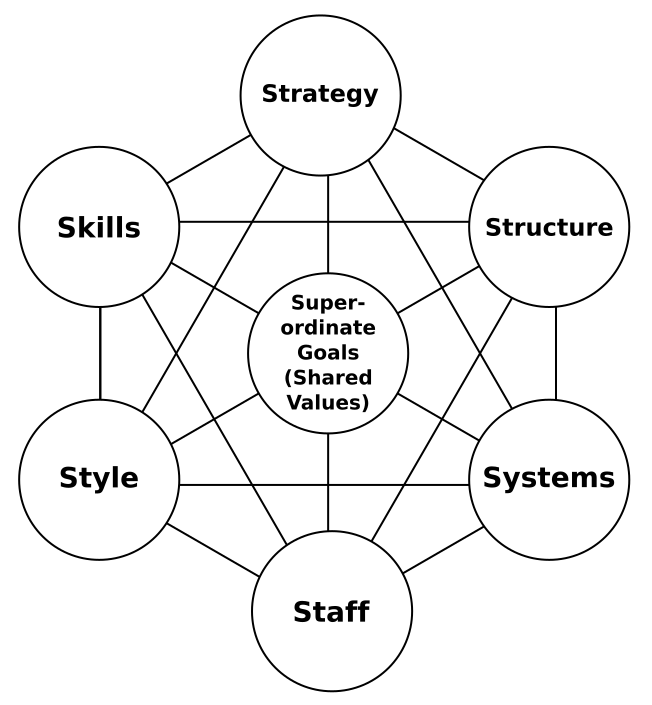
\includegraphics[width=0.6\textwidth]{graphics/sevens_framework}
    \caption{The 7S framework}
    \label{fig:sevens_framework}
\end{figure}

The model emphasises the interdependence of the factors using the connections between them.
One factor may influence others, and all of them must be aligned in order for an organisation to be well organised.
Also, the model is deliberately shaped in a way that does not communicate hierarchy because one factor is not necessarily more important than the others.

A brief explanation of the seven factors in terms of what question(s) each factor tries to answer:

\noindent
\begin{tabular}{>{\bfseries}L{0,2\textwidth} L{0,8\textwidth}}
    Strategy        & What does the organisation do to provide added value? \\
    Skills          & What are the competencies both at the organisation level and the level of its people?\\
    Structure       & How is the organisation arranged?\\
    Style           & How do leaders operate and interact within the organisation?\\
    Systems         & What are the rules, regulations and processes with regard to getting tings done and management activities?\\
    Staff           & How does the organisation make sure it has the right people?\\
    Shared Values   & What are the core beliefs in the organisation about what is important and why the organisation exists?\\
\end{tabular}

\section{Company Analyses and Insights}

\subsection{IKEA}
For our non-software company we have chosen IKEA.
IKEA is primarily known for its self-assembly furniture.
Since 2008, it is the largest furniture retailer in the world, with over 300 stores in business world-wide~\citep{interikea}.

\subsubsection{Approach}
To analyse the IKEA case, at first we did a basic 7S analysis.
This was before the feedback session, during which several major issues were pointed out.
After that, it proved to be difficult to find either reliable or specific sources.
Thus, we had to settle for official sources, interviews, and presentations found on the web in addition to some Harvard Business Review articles.
In order to develop our insights we performed an on-line brainstorm session consisting of two team-members.
We decided to focus on the aspects on \emph{innovation} and \emph{how to get creative work done}.

\subsubsection{Strategy}
\noindent
One of IKEA's fundamental business innovations has been its way of creating value.
Every product is the result of a combination of activities that the business undertakes~\citep{normann1993}.
By optimising the way you combine your activities, you optimise the value you create.

For example, IKEA has innovated in the way it divides its labour.
It engages the customer in the process of manufacturing by means of self-assembly.
IKEA makes every effort to accommodate the customer in this process as much as possible (by distributing catalogues, providing note papers at store entrances, and assisting in self-transportation of the product from the store to the home)~\citep{normann1993}.

Actually, this accommodation should not merely be interpreted as a way of how IKEA creates value for people to consume, but rather as a way of how IKEA tries to mobilise people to create value for themselves by offering services that allow people to easily do the things that they could not before~\citep{normann1993}.

IKEA does this not only on the customer-side but also on the logistics side, by acting as both a customer of and a service-provider to its suppliers~\citep{normann1993}.

This fundamental change in value-creation is why IKEA has become the world's largest furniture retailer~\citep{normann1993}.

\subsubsection{Structure: Business}
IKEA has a complicated, multinational structure.
It is highly decentralised, but it can be said to consist of mainly two parts:
\begin{compactdesc}
    \item[Inter IKEA Systems B.V.] is a franchise company, owner of the \emph{IKEA Concept} (includes IKEA trademarks).
    \item[INGKA Holding B.V.] is the owner of most IKEA stores, which operate under a franchise agreement with Inter IKEA Systems.
\end{compactdesc}
INGKA Holding owns over 300 IKEA stores world-wide; whereas, Inter IKEA Systems owns only one store: IKEA Delft~\citep{interikea}.
%If you have numbers concerning the amount of employees I would put it in here (that way it's consistent with the following section).

\subsubsection{Structure: Development}
IKEA of Sweden AB, in Almhult, Sweden has been commissioned by Inter IKEA Systems to do product development. 
It is the only IKEA store that does product development.

All development is being done on one factory floor with a 4,000 m2 area.
Prototypes of all designs are physically present at this location~\citep{dezeen2015}.

There are about 20 in-house designers, 100 contract-based designers, and 6 scholarships per year.
Design is Agile process: small teams are formed composed of a communicator, a product developer, an engineer (for prototyping), and one or more designers~\citep{dezeen2015}.


\subsubsection{Systems: Business}
Inter IKEA Systems provides the franchisees with the know-how (knowledge, training, standards, etc.) of operations, this is the IKEA Concept.
Proper implementation of the IKEA Concept is the responsibility of the franchisee while Inter IKEA Systems does performance monitoring~\citep{interikea}.

IKEA Delft, the only IKEA store owned by Inter IKEA Systems, is also a test-bed for new ideas and products~\citep{interikea}.

\subsubsection{Systems: Development}
Product design involves visiting people's homes to figure out their needs, so there is some requirements engineering going on~\citep{dezeen2015}.

IKEA sometimes hires well known, expert designers and allows them to create collections in order to learn from their expertise~\citep{dezeen2015}.

\subsubsection{Skills}
Inter IKEA Systems has specialist competence in areas such as~\citep{interikea}:
\begin{compactitem}
    \item Marketing and sales
    \item Retail logistics
    \item Store design and establishment
    \item Communication and interior design
    \item Customer relations
    \item Market research
    \item Competitor monitoring
    \item Market surveillance of new and existing markets
    \item Logistics and media production
\end{compactitem}

\subsubsection{Shared Values: Business}
IKEA remains vague about its core values at the highest level, possibly to remain adaptable.
It does put some emphasis on Swedish culture.
The following values are mentioned on the store websites:
\begin{compactitem}
    \item Leadership by example (management acts according to values)
    \item Constant desire for renewal (adapting to customer needs)
    \item Togetherness and enthusiasm (cooperative problem solving)
    \item Cost-consciousness (low prices)
    \item Striving to meet reality (practicality)
    \item Humbleness and willpower (respect customers and getting things done)
    \item Daring to be different (improve old solutions)
    \item Accept and delegate responsibility (promote people with potential and stimulate them to improve)
    \item Simplicity (easy-going, straightforward approach)
    \item Constantly being "on the way" (continuous improvement)
\end{compactitem}

\subsubsection{Shared Values: Development}
IKEA's development formula is known as \emph{democratic design}.
Democratic design consists of five values~\citep{dezeen2015}:
\begin{compactitem}
    \item Form, the product should look good
    \item Function, the product should meet the need
    \item Quality, the product should not be "cheap"
    \item Sustainability, the product should be designed for long life
    \item Affordability, the product should be affordable for most people
\end{compactitem}

The design should also aim for an authentic Scandinavian style in order to meet the Scandinavian image.
Furthermore, transparency is important during development, so designers can inspire each other.
This is the reason for the factory floor setting~\citep{dezeen2015}.

\subsubsection{Staff}
In order to make sure IKEA has the right people, Inter IKEA Systems provides training and process monitoring.
To what extent the process monitoring is applied to individual co-workers is not known~\citep{franchisorikea}.

Expert designers are sometimes hired in order to learn from~\citep{dezeen2015}.

\subsubsection{Style}
IKEA management \emph{leads by example}~\citep{ikea2016}~\citep{al-hammadi}.
For instance, management does not get first-class plane tickets and expensive hotel rooms.
This reflects the Swedish culture which emphasises simplicity.

\subsubsection{Innovation}

IKEA prides itself on it's innovation but how is the company's innovation achieved? IKEA possesses a flat organisational hierarchy where employees are able to approach upper layers of management. IKEA is also a family company, family companies often try to give their employees a sense of belonging by making them a part of a family. IKEA adopts this practice by calling it's employees coworkers regardless of their rank within the company~\citep{prasant2014}.
Another way to emphasise the (co)workers hierarchy is the idea of "huddle rooms" accepted by the company. These rooms promote idea sharing by employees and increase the idea of belonging~\citep{prasant2014}. While these small measures are just examples of how a company can increase its (co)workers commitment they are powerful motivators if an employee feels part of the family spirit that some family companies posses. 
\paragraph{Innovation} 
IKEA has multiple strategies for innovation, their primary focus for innovation is services and products for their customers. Ideas for innovation for IKEA come from multiple places and even from the organisation itself. IKEA has opened a large innovation lab in Copenhagen to find long term future products ~\citep{fastcodesign2015}. However, IKEA's primary source of ideas comes from the people who know their business the best: the employees. The company has guidelines for its employees where everyone is obligated to contribute ideas on how to improve the business. These ideas are spread throughout the organisation by communication channels and judged whether they have any merit. The way IKEA manages their communication is by managing a large intranet between accessible for all employees around the world. The intranet helps with the promotion of the idea that all coworkers at IKEA are part of the family and their sense of belonging will likely make them loyal and motivated to the company~\citep{bright2015}. Also all the employees will be motivated to help the company grow if they have a sense of belonging to the IKEA family. However, regardless of the validity of ideas IKEA welcomes any and all ideas offered by its employees. The company is convinced that more ideas being discussed will lead to a more active discussion within the company which will in turn lead to more ideas~\citep{fawkes2009}. % sentence above is not that great....


\paragraph{Downsides of the IKEA Model}
With these great company values for employee satisfaction there is also a downside to IKEA's employee policies. Even though the Swedish model claims to have less micro management than other types of company models there is evidence that there is a lot of micro management at IKEA for certain positions. A glance at reviews left by ex workers of IKEA gives a conflicting image~\citep{indeed2016}. Some workers like the management and claim they were taken care of by management while others speak against the management policies at the company. Micro management is contradictory with the values the company likes to present to the outside world where employees are flexible in their working conditions as long as the work gets done on time. There were also several reports over the years of strikes against IKEA because personnel wanted to join a worker's union. This was countered with intimidation and threats to fire them if they were to strike \citep{labornotes2015}\citep{enterprisenews2015}. 

So while the company promotes empowerment by encouraging cooperation among its employees there are a lot of documented instances where the company's values were not applied.  

\subsubsection{Design Process}
The design is a Scrum-like process: small teams are formed composed of a communicator, a product developer, an engineer (for prototyping), and one or more designers.
IKEA has about twenty in-house designers and 100 more on contract.
Combined, they produce around 2,000 designs each year, so this implies that they work on one design for a relatively short amount of time (a few weeks).
All the designers work inside one giant open-space: a 4,000 m2 factory floor where all prototypes of the designs are physically present.
This system stems from a key value during design: transparency, and IKEA believes it inspires designers.
The process also involves visiting people's homes to figure out their needs~\citep{dezeen2015}.

The shared work floor system has some implications that help getting things done.
Namely, the fact that designers share their work with others helps by not only enabling them to get feedback from each other but also enabling them to receive recognition for their work~\citep{belsky2012}.

The Scrum-like process also has benefits for creative work.
Organisation is a key element in the process of bringing ideas to life~\citep{belsky2012}.
First, the Scrum-like structure accommodates the creative process by giving designers a ready-made way to operate, such that they are organised.
Second, there is a sense of responsibility toward others.
Third, there is a presence of leadership (the product developer).
Fourth, it relieves the designers of the interference of every day communication.
These are elements that are all inherent in Scrum as well; therefore, we conclude that Scrum is a good fit for certain elements of a creative process, such as design and perhaps some program design also.

% START OF GOOGLE Section
\subsection{Google}

\subsubsection{Strategy}
In order to sustain its competitive advantage, Google allocates 70\% of its innovation budget to core initiatives, 20\% to neighbouring initiatives and 10\% to transformational initiatives.
Larry Page attributes all of the company's important new product categories to this investment of 10\%.
In 2008 page also stated that even with these investments, 90\% of the employees at Google still focus on more ordinary tasks \citep{Larry64:online}.

Nonetheless, Google is dedicated to keep investing in this area and explore new techniques and methods to change the status quo.
This is not just a strategy that works at Google, there is actual scientific evidence that companies adopting this model perform better \citep{nagji2012managing}.

Another approach to foster innovation is that employees are allowed to spend 20\% of their time on self-proposed projects \citep{Rever82:online}.
In 2013, Google spent 13 billion US dollars on Research and Development, which is roughly 15\% of its revenue \citep{Theto49:online}.

We can conclude that Google does not put all eggs in one basket; it invests a significant amount in moonshot projects, but the focus in the short term is still on its core product offers that generate the current revenue.

\subsubsection{Systems}
In general, Google teams tend to use agile methods.
Some teams adopt XP or Scrum, but there is no company guideline as to which methodology to use.
Most teams are self-organising and are free to choose whatever software processes they see fit.
Teams often do not even have a project manager assigned; teams communicate directly with stakeholders \citep{striebeck2006ssh}.

Google's management does not want to impose methodologies on teams and overburden them.
Management believes that the teams themselves know what processes would work best for them.

The software process is intentionally not centralised, and a person working at Google even claims that Google's philosophy is the exact opposite of something like CMMI \citep{W66:online} that requires certain processes to be put in place.
If one team discovers that a certain practise works well for them, other teams will follow \citep{striebeck2006ssh}.
Thus, there is a lot of experimentation going on at any point in time.

The AdWords team is the exception to this philosophy, in that more standards are imposed on the process employed.
This is because AdWords is much more business input driven than other projects.
The AdWords project does have project managers and a fairly large management team.
Some projects tried to use Agile practises, but not every practice was introduced at the same time.
Team members needed to become accustomed and see the benefit of a certain practice before others are introduced.
Post-mortems are conducted at the end of a project, and positive and negative points of certain methodologies are reviewed in order to decide which practises should be employed in future projects.
Certain practises can be modified or improved based on this feedback.
Slowly, some teams that were initially reluctant to adopt formal software processes saw the value of using certain Agile practises.

Peer reviewing is required for all code written \citep{Steve4:online}. When it comes to writing code, engineers are very disciplined. The result is that the whole codebase looks the same, so it is easier for people to switch teams.

\subsubsection{Structure}
The organisational structure of Google can be classified as a matrix organisation, although it is one with a rather flat hierarchy.
Teams are assigned by function and by product.
For example, a web developer is assigned to the Engineering \& Design team \citep{Teams23:online}, as well as the Google+ team.
Google's organisational structure is relatively flat.
That is, there hardly is any middle management and upper management can be approached quite easily.

\subsubsection{Skills}
In the past, Google, as a company, excelled at quick decision making.
When Larry Page took over as CEO in 2012 and reformed decision making at the company \citep{Start62:online}, he believed that as the company had grown, it had become less agile \citep{Profe61:online}.

Another area of competence is the way Google approaches testing.
Traditionally, software companies employed testers who solely had to test the software developers wrote.
Google does not believe in this approach, and for this reason Google does not have a 'testing department' \citep{Googl3:online}.
Rather, there are supporting teams that can temporarily embed employees in project teams to provide them tools, techniques and other guidance related to testing.
Development teams are required to develop tests themselves.
This approach has led to success for Google, turning each developer into a tester.
This is compatible to the way testing is done in Scrum teams; since the focus is on delivering working software, testing is usually incorporated in the sprints rather than doing it afterwards.

Finally, as highlighted in the 'strategy' section, Google has achieved significant success with taking bold risks fostered by its drive on innovation.
This drive and the execution of it can be considered a corporate skill.

\subsubsection{Shared Values}
As of 2016, Google has the following mission: ``to organise the world’s information and make it universally accessible and useful.'' \citep{About86:online}.
Google encourages risk taking, non-traditional thinking, and innovation by employees \citep{Decis25:online}.
In addition, Google deeply values integrity, collaboration, and trust \citep{striebeck2006ssh}.
The following quotes convey those shared values: ``When a vice president in charge of the company’s advertising system made a mistake costing the company millions of dollars and apologised for the mistake, she was commended by Larry Page, who congratulated her for making the mistake and noting that he would rather run a company where they are moving quickly and doing too much, as opposed to being too cautious and doing too little.'' and ``Please fail very quickly - so you can try again'' \citep{ORGAN15:online}.
Thus, making mistakes is accepted, and agility is a shared value.

This has consequences for the software processes in place at the company.
After all, a new process, such as Scrum, may be experimented with on a small scale to see if it works out and the rest of the company should adopt it.
Founder Sergey Brin states that the company's culture should not be static; it should continuously improve.
This may facilitate adoption of new software processes. Google has even appointed a 'chief culture officer' to guide this.

\subsubsection{Staff}
Google's hiring policy is that they only recruit the brightest and best individuals. In terms of Etzioni's compliance theory \citep{lunenburg2013compliance}, Google can be classified as being a Normative-Moral organisation when considering the type of power they use to direct the behaviour of their members and the type of involvement of the participants. Normative because most employees share the vision to innovate and passion for the company to succeed and change the state of technology. Moral because employees are proud to work at Google and are often loyal to the company, staying with the company for years at end.

\subsubsection{Style}
It is publicly known that Google values decisions made by teams \citep{ORGAN15:online}, as opposed to decision making by single individuals.
Until recently, high-level decisions were made consensually by founders Larry Page and Sergey Brin, accompanied by CEO Eric Schmidt.
Google does not enforce decision making in a top-down way.
Rather, it stresses the importance of rational persuasion, and teams may propagate these decisions bottom-up.
Amit Singh (Google's senior vice-president and head for worldwide enterprise services) states: ``We believe in bottoms-up decision making'' \citep{Googl11:online}.
It is also believed that top-down decision making leads to organisational anarchy.
The emphasis here is on rational, thus every decision should involve proper argumentation and should not be based on instinct or feeling.
In addition, employees at Google usually work in open office environments.
The reason behind this is the conviction that open offices foster teamwork.

% END OF GOOGLE SECTION

\section{Lessons Learned}

% What can you learn from this about the method RUP?
\subsection{RUP}
As is the case with Scrum, RUP in its ideology is meant to be adapted to the implementing organisation.
Rather than trying to work around certain elements of a methodology, trying to determine why it doesn't work for the organisation and the accompanying rationale is what is highly valuable from a project management standpoint.
There is no single methodology that provides it all, you just have to find out what works and elaborate upon that.

% What can you learn from this about the method Scrum?
\subsection{SCRUM}
As mentioned earlier, Google employs agile software processes but in their own way.
Steps can be adapted when implementing them in the organisation in the spirit of the agile manifesto, and teams are one step at a time convinced of the advantages of using certain Scrum practises, such as the daily scrum stand-up meeting.
If team members dislike a certain part of the methodology, these employees have the freedom to diverge from it.
The methodology is not forced upon the engineers by upper management, rather the engineers must discover the advantages it brings themselves and see if its worth it.
The lessons learned is that Scrum should not been as some doctrine, but can be implemented differently in an organisation if there are good reasons for doing this.

IKEA perhaps uses a Scrum-like process for design itself; however, the total process for product development contains a requirements and QA phase as well, at the Inter IKEA Systems, Delft store.
Thus, it seems that Scrum can be successfully incorporated in product development for these kinds of products, but it might not be self-sufficient when you're mass-manufacturing even for relatively simple products.
This might be because IKEA is not a software company, you cannot just patch a chair.
Hence the additional QA process: bugs in software cause patches which are cheap to distribute, bugs in hardware cause recalls which are expensive transport wise.

% What can you learn from this for your failed case? 
\subsection{Failed Case}
We can't be sure since the amount of information regarding the Ariane 5 project is limited, but we suspect that some engineers have issued warnings on the redundancy of the system and the decisions made.
Compiler warnings given should have made the engineers aware of this risk.
In Ariane 5 decisions were made quite top-down. From Google's approach we can learn that in some cases it works great to give autonomy to teams.
It also shows us that a bottom-up approach works in the case of a technological company, so it could work for ESA as well.
What does need to be stressed is that decisions should be made in a rational way, preferably backup up by, for example, quantitative evidence.
No decisions should be made based on gut feeling.

Comparing IKEA and the Ariane 5 project is very difficult.
First, because IKEA's products are relatively very simple.
One practice that could have helped the Ariane 5 is the hiring of experts.
For example, if the team had asked an experienced engineer from NASA to do an audit, this engineer would have pointed out that NASA also designs for robustness on the software side.

\section{Conclusion}
Both Google and IKEA apply RUP/Scrum in their own context.
They do not see these processes as good fits for every situation, so they acknowledge that the context of the process is important, and they adapt the processes.
This last part is perhaps the most notable takeaway.